\paragraph{ANOVA}
%\subparagraph{Predictors with only 2 levels}
%One way of formulating the common-slope model is :
%$$ Y_{i} = \alpha + \beta X_{i} + \gamma D_{i} + \epsilon_{i}$$ where $D$, called a dummy-variable
%regressor or indicator variable, $$D1=
%\begin{cases}
%	1\text{ for women}\\
%	0\text{ for men}
%\end{cases}
%$$
%\begin{figure}[H]
%	\begin{center}
%		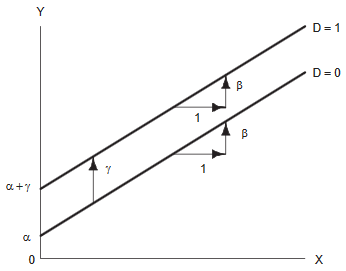
\includegraphics[width=.3\textwidth]{./chap/1chap/2sec/3images/1_graphicalDummy.PNG}
%	\end{center}
%	\caption{The parameters in the additive dummy-regression model}
%	\label{fig:1_graphicalDummy}
%\end{figure}
%
%\emph{gender} is a qualitative explanatory variable, with categories \emph{male} and \emph{female}
%the dummy variable $D$ is a regressor representing the explanatory variable gender.
%\subparagraph{Modelling interactions}
%$$ Y_{i} = \alpha + \beta X_{i} + \gamma D_{i} + \delta X_{i}D_{i} + \epsilon_{i}$$
%
%\begin{figure}[H]
%	\begin{center}
%		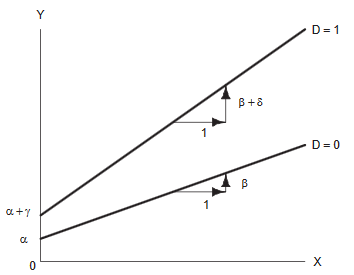
\includegraphics[width=.3\textwidth]{./chap/1chap/2sec/3images/2_graphicDummyInteract.PNG}
%	\end{center}
%	\caption{The parameters in the dummy-regression model with interaction}
%	\label{fig:1_graphicalDummy}
%\end{figure}

\subparagraph{ANOVA models}
Analysis of Variance describes \sB{the partition of the response variable sum of squares in a 
linear model into ``explained'' and ``unexplained'' components.}\\
\begin{itemize}
	\item Single categorical explanatory variable corresponds to One-Way ANOVA
	\item 2 factors to Two-Way ANOVA
	\item 3 factors to Three-Way ANOVA
\end{itemize}

\subparagraph{\emph{One-way} ANOVA}
\tR{examines equality of population means for a quantitative outcome and a 
single categorical explanatory variable with any number of levels}.\\
The term \tB{``one-way'' indicates that there is a single explanatory variable (``treatment'') 
with 2 or more levels and only one level of treatment is applied at any time for a given subject}.
\\
The term ``analysis of variance'' is a bit of misnomer, \tB{we use variance-like quantities to
study the equality or non-equality of population means}, so we are analyzing means, not variances.

\begin{center}
	The statistical model for which one-way ANOVA is appropriate is that the
	\begin{itemize}
		\item (Quantitative) Outcomes for each group are normally distributed
		\item Outcome variances are all equal to  ($\sigma^{2}$)
		\item The errors are assumed to be independent.
	\end{itemize}
\end{center}

\begin{center}
	\enc{$H_{0}:\forall (i,j) \in \inter{1}{k}^{2} \mu_{i} = \mu_{j}$}
\end{center}

In ANOVA \sB{we work with variances and also ``variance-like quantities'' which are not really the
variance of anything}, but are still calculated as $\frac{SS}{df}$ all of these quantities are
called ``mean squares''.\\

The deviation for subject $j$ of group $i$ in the figure above is mathematically equal to $Y_{ij}-
\overline{Y}_{i}$ where $Y_{ij}$ is the observed value for subject $j$ of group $i$ and $\overline{Y}_{i}$ is the sample mean for group $i$.
\begin{figure}[H]
	\begin{center}
		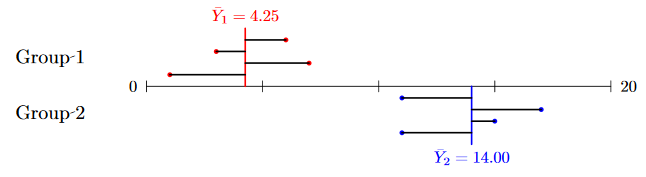
\includegraphics[width=\textwidth]{./chap/1chap/2sec/3images/3_anovaInterGrp.PNG}
	\end{center}
	\caption{Deviations for within-group of squares}
	\label{fig:3_anovaInterGrp}
\end{figure}
\begin{center}
\enc{
$ MS_{within} = \dfrac{SS_{within}}{df_{within}}
\begin{cases}
	SS_{within} = \su{{j=1}}{k}SS_{j}=\su{{j=1}}{k}\su{{i=1}}{n_{j}}\left(Y_{ij}-\overline{Y}_{\bullet j}
	\right)\\
	df_{within} = df_{j} = \su{{j=1}}{k}(n_{j}-1) = N-k
\end{cases}
$
}\end{center}

\tB{$MS_{within}$ is a good estimate of $\sigma^{2}$ from our model regardless of the truth of 
$H_{0}$.} This is due to the way $SS_{within}$ is defined.

\begin{figure}[H]
	\begin{center}
		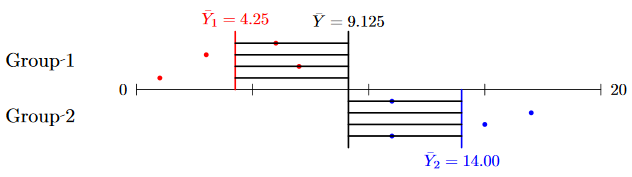
\includegraphics[width=\textwidth]{./chap/1chap/2sec/3images/4_anovaBtw.PNG}
	\end{center}
	\caption{Deviations for betwwen-group sum of squares}
	\label{fig:4_anovaBtw}
\end{figure}
$SS_{between}$ is the sum of the $N$ squared between-group deviations, where the deviation is
the same for all subjects in the same group. The formula is : 
\begin{center}
\enc{
$
MS_{Between} = \dfrac{SS_{Between}}{df_{between}}
\begin{cases}
SS_{between} = \su{{j=1}}{k}n_{j}\left(\overline{Y}_{\bullet j}-\overline{Y}\right)^{2}\\
df_{between} = k-1
\end{cases}
$
}\end{center}
Because of the way $SS_{between}$ is defined, \tB{$MS_{between}$ is a good estimate of $\sigma^{2}
$ only if $H_{0}$ is true}. Otherwise it tends to be larger. \\
The $F-statistic$ defined by $F=\dfrac{MS_{between}}{MS_{within}}$ \sR{tends to be larger if the
alternative hypothesis is true than if the null hypothesis is true}.\\

We can quantify ``large'' for the \emph{F-statistic}, by comparing it to its null sampling 
distribution which is the specific \emph{F-distribution}  which has degrees of freedom matching
the numerator and denominator of the \emph{F-statistic}.\\
Concerning inferences to build the confidence interval we need the \tB{\emph{standard error} (the
standard deviation of the means) that is $\sqrt{\dfrac{MS_{within}}{n_{i}}}$}\\

Numerically we have:\\
Given 2 samples with means $\mu_{1}$ and $\mu_{2}$, same variance $\sigma^{2}$ and $n=n_{1}+n_{2}$
observations.
Model: 
\begin{center}
	$\forall (j,i)\in\inter{1}{2}\times\inter{1}{n_{j}}y_{ij} = \mu_{i} + \epsilon_{ij} = \mu + \alpha_{j} + \epsilon_{ij}$
\end{center}
$\alpha_{j}=\mu_{j}-\mu$ is called (treatment-) effect

Decomposition:
\begin{align*}
	SS_{total} =& \su{{j=1}}{n_{1}}\left(y_{1j}-\overline{y}\right)^{2} +
	\su{{j=1}}{n_{2}}\left(y_{2j}-\overline{y}\right)^{2}\\
	=& \su{{j=1}}{n_{1}}\left(y_{1j}-\overline{y_{1}}+\overline{y_{1}}-\overline{y}\right)^{2}
	+ \su{{j=1}}{n_{2}}\left(y_{2j}-\overline{y_{2}}+\overline{y_{2}}-\overline{y}\right)^{2}\\
	=& \underbrace{(n_{1}-1)s_{1}^{2} + (n_{2}-1)s_{2}^{2}}_{SS_{within}} +
	\underbrace{n_{1}(\overline{y}_{1}-\overline{y}) + 
	n_{2}(\overline{y}_{2})-\overline{y}^{2}}_{SS_{between}}
\end{align*}
$SS_{between}$ corresponds to squared enumerator $(\overline{y}_{1} - \overline{y}_{2})^{2}$ of
the statistic: 
\begin{align*}
	SS_{between} =& n_{1}(\overline{y}_{1}-\overline{y})^{2} + 
	n_{2}(\overline{y}_{2}-\overline{y})^{2}\\
	=& n_{1}\left(\overline{y}_{1}-\dfrac{n_{1}\overline{y}_{1}+n_{2}\overline{y}_{2}}{n_{1}+
	n_{2}}\right)^{2} + n_{2}\left(\overline{y}_{2}-\dfrac{n_{1}\overline{y}_{1}+n_{2}
	\overline{y}_{2}}{n_{1}+ n_{2}}\right)^{2}\\
	=& \dfrac{n_{1}n_{2}}{n_{1}+n_{2}}\left(\overline{y}_{1}-\overline{y}_{2}\right)^{2}
\end{align*}
$SS_{within}$ corresponds to denominator of \emph{t-statistic}:
$s=\sqrt{\dfrac{(n_{1}-1)s_{1}^{2}+(n_{2}-1)s_{2}^{2}}{n_{1}+n_{2}-2}}$\\
Pooled variance that is an estimate of the fixed common variance $\sigma^{2}$ underlying various
populations that have different means.
$\hat{\sigma}=\dfrac{(n_{1}-1)s_{1}^{2}+(n_{2}-1)s_{2}^{2}}{(n_{1}-1)+(n_{2}-1)}$
Null hypothesis $H_{0}:\mu_{1}=\mu_{2}$ or $\alpha_{1}=\alpha_{2}=0$
\emph{F-test}
$\left(\overline{Y}_{1}-\overline{Y}_{2}\right)\hookrightarrow \mathcal{N}\left(\mu_{1}-\mu_{2},
\left(\frac{1}{n_{1}}+\frac{1}{n_{2}}\right)\sigma^{2}\right)\\
\E{\left[\overline{Y}_{1}-\overline{Y}_{2}\right]^{2}}=\left(\frac{1}{n_{1}}+\frac{1}{n_{2}}
\right)\sigma^{2}+(\mu_{1}-\mu_{2})^{2}\\
\E{MS_{between}}=\E{\frac{n_{1}n_{2}}{n_{1}+n_{2}}\left[\overline{Y}_{1}-\overline{Y}_{2}
\right]^{2}} = \sigma^{2}+\frac{n_{1}n_{2}}{n_{1}+n_{2}}(\mu_{1}-\mu_{2})^{2}\\
\E{MS_{whithin}}=\sigma^{2}\\
F = \dfrac{MS_{between}}{MS_{within}}$
Here $F=t^{2}$\\
\begin{align*}
	\text{Degrees of freedom} =& n - 1\\
	=& \underbrace{(n-m)}_{df_{within}} + \underbrace{(m-1)}_{df_{between}}
\end{align*}
\begin{itemize}
	\item $SS_{within}$ and $SS_{between}$ are independent
	\item under $H_{0}$ $\E{MS_{between}} = \E{MS_{within}} = \sigma^{2}$
	\item under $H_{a}$ $\E{MS_{between}}>\sigma^{2}$ and $\E{MS_{within}} = \sigma^{2}$
\end{itemize}
Hence $$ F= \dfrac{MS_{between}}{MS_{within}}\hookrightarrow F_{m-1,n-m}$$
In the case of 2 groups (``\emph{t-test}'') we received:
$$ \overline{y}_{1}-\overline{y}_{2} \pm t_{n-2,1-\frac{\alpha}{2}}s\sqrt{\frac{1}{n_{1}}+
\frac{1}{n_{2}}}$$
\subparagraph{Two-way-ANOVA}
If a quantitative explanatory variable is also included, that variable is usually called a 
\emph{covariate}.\\
The usual assumptions of normality, equal variance and independent errors apply.\\

\tB{ANOVA decomposes the total variance} present in the data into contribution of the single 
sources of variation :
\begin{itemize}
	\item \tB{systematic contribution}: differences of means
	\item \tB{random rest}: variability around group mean
\end{itemize}
We have the total variance law:
\begin{center}
\enc{
$
\begin{cases}
X\& Y\text{ random variables on the same probability space}\\
\text{variance of }Y\text{ is finite}
\end{cases}\Rightarrow
\V{Y} = \E{\mathbb{V}\left(Y|X\right)} + \V{\mathbb{E}\left(Y|X\right)}
$}
\end{center}

Numerically:
$$\forall (i,j,k)\in\inter{1}{m_{1}}\times\inter{1}{m_{2}}\times\inter{1}{n_{ij}}~y_{ijk} =
\mu_{ij} +\epsilon_{ijk},~\epsilon_{ijk}\hookrightarrow \mathcal{N}(0,\sigma^{2})$$
Decomposition of means:
\begin{align*}
	\mu_{ij} &= \mu + (\mu_{i}-\mu) + (\mu_{j}-\mu) + (\mu_{ij}-\mu_{j}-\mu_{i}+\mu)\\
	&= \mu +\alpha_{i} +\beta_{j} + \gamma_{ij}\\
	&= \text{``overall mean''} + \text{``main effect of A''} + \text{``main effect of B''} +
	\text{``interaction of A and B''}
\end{align*}
Null hypothesis:
\begin{itemize}
	\item All $\alpha_{i}=0$
	\item All $\beta_{j}=0$
	\item All $\gamma_{ij}=0$
\end{itemize}

\begin{python}
import statsmodels.api as sm

data = pd.read_csv('myFile.csv', sep=',')
model = sm.ols('y ~ C(X1, Sum)*C(X2, Sum)', data=data).fit()
table = sm.stats.anova_lm(model, typ=2) # typ=2 indicates that we are testing for each main effect
# after the other main effect.
print(table)
\end{python}

\paragraph{ANCOVA} The multiple regression model below would be equal to an ANCOVA, if \sB{$X_{1}$ was binary and $X_{2}$ was some covariate of interest}:$y = \beta_{0}+\beta_{1}X_{1}+\beta_{2}X_{2}+\epsilon$\\ The key is in the interpretation of the intercept value and the slope for the binary predictor.  If $X_{1}$ is binary with values 0 and 1, then the \begin{itemize} \item \textbf{\emph{intercept}} is the average of \tB{$\beta_{0}=\E{y|(X_{1},X_{2})=(0,0)} $} \item \textbf{\emph{slope}} represents the mean difference between 0 and 1 group\\ \tB{$\beta_{1} = \E{y|(X_{1},X_{2})=(1, x_{2})}-\E{y|(X_{1},X_{2})=(0, x_{2})}$}
\end{itemize}

\subparagraph{When is ANCOVA used?}
It is usually used for analysis of quasi-experimental studies, when the regression groups are
not randomly assigned and the researcher wishes to statically ``equate'' groups on one or more
variables which may differ across groups. 
\subparagraph{Relation to Repeated Measures ANOVA}
The repeated measures ANOVA (and the paired t-test) is equivalent to test if the average 
difference score is different from zero. However ANCOVA and Repeated Measures ANOVA tests are not
equivalent, because they represent 2 different ways of conceptualizing change.
\subparagraph{Adjusted Means} 
ANCOVA procedures will produce adjusted means, which represents the means of each group once the
covariate(s) has been controlled.\\ In Regression terms, these adjusted means come from the 
intercept: $\beta_{0}=\overline{y}-\beta_{1}\overline{X}_{1}-\beta_{2}\overline{X}_{2}$
\sB{Because the intercept represents the average value of $y$ when all predictors equal zero, we 
have to pay attention to the scaling of the variables.} If the grouping variable, $X_{1}$, has two
values 0 and 1, the adjustment leads to an intercept for the 0 group where the covariate, $X_{2}$,
is also equal zero. In many cases, the estimated mean when covariates are equal to zero is not
meaningful. So if using regression analysis and there is interest in obtaining the adjusted means,
\tB{it is common to rescale the covariates, $x_{2}=X_{2}-\overline{X}_{2}$}.\\
Then in regression analysis, the adjusted means can be computed by using the regression 
coefficients and inserting values for $X_{1}$\\ $\overline{Y}_{adj}=\beta_{0}+\beta_{1}X_{1}-\beta_{2}\overline{X}_{2}$

\subparagraph{Should I use ANCOVA or Regression?}
Test hypothesis about group differences using an ANCOVA procedure or a regression analysis will 
give the same result, when there are several categories for the independent variable or 
interactions are of interest we should use ANCOVA. 
\subparagraph{Sum of Squares}
The issue type  of sum of squares comes up in ANCOVA as it does in ANOVA: 

\begin{itemize}
	\item[Type \textbf{I}:] Each effect partials out or controls for only those effect
		entered before it. If effect $A$ is entered first, it does not partial out $B$ or 
		$A\times B$ added after it. But $B$ can partial out $A$, and interaction $A\times
		B$ partials out $A$ and $B$
	\item[Type \textbf{II}:] Each effect at the same step or before is controlled but not for
		later steps. Say $A$ and $B$ are entered first and then $A\times B$ is added. $A$
		controls for $B$ and $B$ controls for $A$. Neither controls for $A\times B$, but
		$A\times B$ controls for both $A$ and $B$.
	\item[Type \textbf{III}:] adjusts fro all other factors or variables in the model. 
\end{itemize}

\emph{R code}
\begin{rcode}[deletekeywords={model, df}]
model_ancova <- aov('y ~ f1 + f2*x1', data=df)
print(summary(model_ancova))
\end{rcode}

